\begin{figure}[htp]
  \centering
  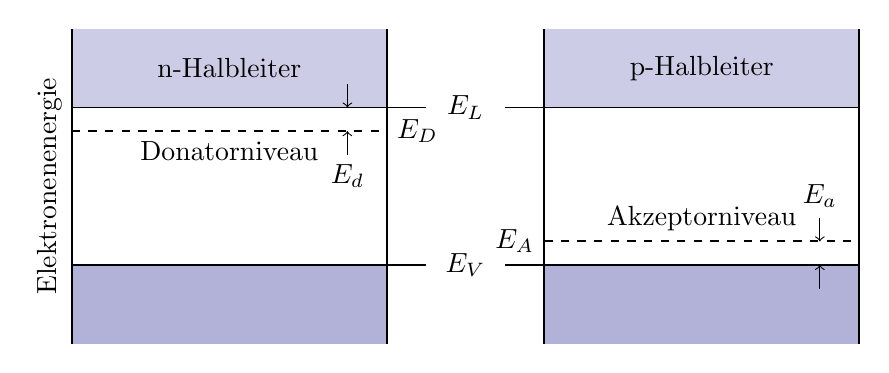
\begin{tikzpicture}
    \fill[fill=black!50!blue, fill opacity = 0.2] (0,4) rectangle (4,3);
    \fill[fill=black!50!blue, fill opacity = 0.3] (0,0) rectangle (4,1);
    \fill[fill=black!50!blue, fill opacity = 0.2] (6,4) rectangle (10,3);
    \fill[fill=black!50!blue, fill opacity = 0.3] (6,0) rectangle (10,1);
    \draw[thick] (0,0) --node[rotate=90, above]{Elektronenenergie} (0,4);
    \draw[thick] (4,0) -- (4,4);
    \draw[thick] (6,0) -- (6,4);
    \draw[thick] (10,0) -- (10,4);
    \node (A) at (2,3.5){n-Halbleiter};
    \node (A) at (8,3.5){p-Halbleiter};
    \draw[thick, dashed] (0,2.7) --node[below]{Donatorniveau} (4,2.7)node[right]{$E_D$};
    \draw[thick, dashed] (6,1.3)node[left]{$E_A$} --node[above]{Akzeptorniveau} (10,1.3);
    \draw (0,3)-- (4.5,3);
    \draw (5.5,3)-- (10,3);
    \node (A) at (5,3){$E_L$};
    \draw (0,1)-- (4.5,1);
    \draw (5.5,1)-- (10,1);
    \node (A) at (5,1){$E_V$};
    \draw[->] (3.5,3.3) -- (3.5,3);
    \draw[->] (3.5,2.4)node[below]{$E_d$} -- (3.5,2.7);
    \draw[->] (9.5,1.6)node[above]{$E_a$} -- (9.5,1.3);
    \draw[->] (9.5,0.7) -- (9.5,1);
  \end{tikzpicture}
  \caption{Störstellenniveaus im Halbleiter. Der Grundzustand $E_D$ der Donatoren liegt knapp unterhalb der Leitungsbandkante. Die Ionisierungsenergie der Elektronen beträgt $E_d$. Der Grundzustand der Akzeptoren befindet sich knapp oberhalb der Valenzbandkante. Die Ionisierungsenergie der Löcher ist $E_a$. Abbildung nach~\cite{Hunklinger}.}
  \label{fig:Störstellenniveaus}
\end{figure}
